%%=============================================================================
%% Resultaten
%%=============================================================================

\chapter{\IfLanguageName{dutch}{Resultaten}{Results}}%
\label{ch:resultaten}

\section{\IfLanguageName{dutch}{Inleiding}{Introduction}}
\label{sec:inleiding-resultaten}

In sectie~\ref{sec:evaluatie-criteria} was sprake over feedback van de werknemers van Evolane.
Vermits Netskope tijdens de evaluatieperiode al reeds in gebruik was, moet de DLP-oplossing hierop verder bouwen.
Tijdens de eerste weken van de evaluatieperiode was het initieel het doel om de geïmplenteerde DLP-regels van \texttt{User Alert} naar \texttt{Block} te zetten.
% Tijdens de eerste weken was het initieel het doel om de DLP-regels van \textit{User-Alert} naar \textit{Block} te zetten.
% Maar omdat Netskope bij veel werknemers uitstond door een slechte configuratie van voordien, is hier ook geen verdere feedback op gekomen.
Aangezien Netskope bij veel werknemers reeds vooraf uitstond door een niet optimale configuratie, werd hierop geen verdere feedback gegeven.
Netskope zorgde bijvoorbeeld ervoor dat security werknemers klanten-websites niet konden troubleshooten, \texttt{dig} werkte niet altijd, enzovoort.
Gedurende de momenten dat Netskope wel het verkeer verwerkte, werden een aantal incidenten vastgesteld.
De incidenten waren voornamelijk klantendocumenten die over Slack en e-mail werden verstuurd. 
Deze incidenten stelden wel vast dat het \textit{Security} team van Evolane heel andere confidentiële data verwerkt, vergeleken met het \textit{Sales} team.

\section{\IfLanguageName{dutch}{Incidenten}{Incidents}}
\label{sec:incidenten-resultaten}

Van de \textbf{63.523} verstuurde berichten onderschepte Netskope \textbf{15.088} incidenten, wat neerkomt op 19,17\% van de berichten~\ref{fig:pie-message-vs-incident}.
Het verstuurde aantal berichten correspondeert met \textbf{21} eindgebruikers van \textit{Enron}. 
% % % % Nog te noteren hoeveel users in deze berichten zaten


\begin{figure}[H]
  \centering
  \begin{tikzpicture}
    \pie[
      radius=2.5,
      text=legend,
      before number=,
      after number=\%,
      sum=auto,
      color={Blauw, Rood, HogentOranje, Groen, Paars}
    ]{
      80.83/Verstuurde e-mails (\textbf{63.523} - 80.83\%),
      19.17/Gedetecteerde incidenten (\textbf{15.088} - 19.17\%)
    }
  \end{tikzpicture}
  \caption{Total messages vs detected incidents}
  \label{fig:pie-message-vs-incident}
\end{figure}

In figuur~\ref{fig:netskope_user_info} staan alle incidenten weergegeven voor de eindgebruiker die tijdens de evaluatieperiode het script heeft uitgevoerd.
De gemeten incidenten zijn gebeurd door middel van \texttt{POST}-requests, de \textit{Download Bytes} zijn hierdoor niet relevant.
Er zijn voor \textit{Upload Bytes} ongeveer \textbf{338 MB} aan data verstuurd, wat overeenkomt met \textbf{63.523} berichten. 
De overige 101.5 MB zijn afkomstig van extra testen of dubbele data. 
Het aantal bezochte websites kwam in totaal op \textbf{33}, aangezien de \textit{\textbf{gehashte}} \gls{url} \texttt{https://<hash>.ngrok-free.app} 
na elke opstart van het script vernieuwde~\ref{subsubsec:ngrok-webinterface}.

\begin{figure}[H]
    \centering
    \scriptsize
    \includegraphics[width=0.99\textwidth]{img/user_info.png}
    \caption{Gebruikersinformatie van Netskope DLP}
    \label{fig:netskope_user_info}
\end{figure}

\subsection{\IfLanguageName{dutch}{Incidenten aan de hand van risicoscore}{Incidents based on risk score}}
\label{subsec:incidenten-risicoscore}

Van de \textbf{15.088} e-mail-incidenten waren in totaal \textbf{306.403} overtredingen.
Het \texttt{Predef\-ined-DLP}\--beleid bevat alle vooraf gedefinieerde DLP-regels van Netskope, waar de threshold op een onaanpasbare waarde staat~\ref{tab:risico_thresholds}.
Dit houdt in dat de incidenten niet overeenkomen met de door dit onderzoek geconfigureerde thresholds.
Aangezien bij \textbf{één} overtreding een incident aangemaakt wordt, kan wel een tweede cirkeldiagram~\ref{fig:pie-severity-dlp-custom-rules} worden opgesteld, die de verdeling van de incidenten weergeeft.
Dit cirkeldiagram is gebaseerd op de gerapporteerde incidenten van Netskope. 
Hiervan wordt het aantal \textbf{overtredingen} \textbf\textit{{per DLP-regel per e-mail}} geanalyseerd om dit dan te corresponderen aan de geschikte thresholds van tabel~\ref{tab:risico_thresholds} uit hoofstuk~\ref{ch:risicoanalyse}.
Deze analyse wordt uitgevoerd door al de incidenten van Netskope te filteren op basis van het aantal overtredingen die per DLP-regel zijn gevonden, zoals te zien in tabel~\ref{tab:fullname-near-ssn}.
In totaal waren \textbf{72} unieke DLP-regels geregistreerd door Netskope.

\begin{table}[h!]
  \centering
  \small
  \scriptsize
  \begin{tabular}{lcc}
    \toprule
    \textbf{Regelnaam} & \textbf{Aantal overtredingen} & \textbf{Aantal keer gedetecteerd} \\
    \midrule
    FullName-Near-SSN-Unique & 2 & 6 \\
    FullName-Near-SSN-Unique & 4 & 3 \\
    \bottomrule
  \end{tabular}
  \caption{Aantal overtredingen voor regel \texttt{FullName-Near-SSN-Unique}}
  \label{tab:fullname-near-ssn}
\end{table}

Figuur~\ref{fig:pie-severity} toont de verdeling van de incidenten op basis van hoe Netskope deze heeft geclassificeerd.
% Figuur~\ref{fig:pie-severity} toont de verdeling van de incidenten op basis van de hoe ze door Netskope zijn geclassificeerd. 
De verdeling van de percentages van de incidenten staat in tabel~\ref{tab:severity-comparison} weergegeven.
Figuur~\ref{fig:pie-severity-dlp-custom-rules} kan mogelijks afwijken, mocht deze test opnieuw uitgevoerd worden.


% Low: 172512 violations
% Medium: 111236 violations
% High: 22630 violations
% Critical: 25 violations

% \begin{figure}[H]
%   \centering
%   \begin{tikzpicture}
%     \pie[
%       radius=3,
%       text=legend,
%       before number=,
%       after number=\%,
%       sum=auto,
%       color={Rood, HogentOranje, Blauw, Groen, Paars}
%     ]{
%       0.01/Critical (\textbf{25} - 0.01\%),
%       7.39/High (\textbf{22630} - 7.39\%),
%       36.30/Medium (\textbf{111236} - 36.30\%),
%       56.30/Low (\textbf{172512} - 56.30\%)
%     }
%   \end{tikzpicture}
%   \caption{Severity van incidenten}
%   \label{fig:pie-severity}
% \end{figure}

\begin{figure}[H]
  \centering
  \begin{minipage}{0.45\textwidth}
    \centering
    \small
    \begin{tikzpicture}
      \pie[
        radius=2,
        text=legend,
        before number=,
        after number=\%,
        sum=auto,
        color={Rood, HogentOranje, Blauw, Groen}
      ]{
        0.01/Critical (0.01\%),
        7.39/High (7.39\%),
        36.30/Medium (36.30\%),
        56.30/Low (56.30\%)
      }
    \end{tikzpicture}
    \caption{Netskope's incident risicoscore (originele threshold)}
    \label{fig:pie-severity}
  \end{minipage}
  \hfill
  \begin{minipage}{0.45\textwidth}
    \centering
    \small
    \begin{tikzpicture}
      \pie[
        radius=2,
        text=legend,
        before number=,
        after number=\%,
        sum=auto,
        color={Rood, HogentOranje, Blauw, Groen}
      ]{
        4.94/Critical (4.94\%),
        17.82/High (17.82\%),
        41.03/Medium (41.03\%),
        36.21/Low (36.21\%)
      }
    \end{tikzpicture}
    \caption{Eigen gedefinieerde incident risicoscore, gebaseerd op risicoscore~\ref{tab:risico_thresholds}}
    \label{fig:pie-severity-dlp-custom-rules}
  \end{minipage}
\end{figure}

\begin{table}[H]
  \centering
  \scriptsize
  \begin{tabular}{lrrrr}
    \toprule
    \textbf{Severity} & \textbf{Aantal (Origineel)} & \textbf{\% (Origineel)} & \textbf{Aantal (Geoptimaliseerd)} & \textbf{\% (Geoptimaliseerd)} \\
    \midrule
    Low       & 172.512 & 56.30\% & 110.983 & 36.21\% \\
    Medium    & 111.236 & 36.30\% & 125.657 & 41.03\% \\
    High      &  22.630 &  7.39\% &  54.622 & 17.82\% \\
    Critical  &     25 &  0.01\% &  15.141 &  4.94\% \\
    \midrule
    \multicolumn{5}{r}{\textbf{Totaal aantal overtredingen: 306.403}} \\
    \bottomrule
  \end{tabular}
  \caption{Vergelijking van incident risicoscore (originele threshold~\ref{fig:pie-severity} vergeleken met eigen gedefinieerde threshold~\ref{fig:pie-severity-dlp-custom-rules})}
  \label{tab:severity-comparison}
\end{table}

Hierbij valt op dat de \textit{Critical} incidenten in de originele configuratie slechts 0.01\% van de incidenten zijn~\ref{fig:pie-severity}, terwijl dit in de geoptimaliseerde configuratie 4.94\% is~\ref{fig:pie-severity-dlp-custom-rules}. 
Doordat de threshold van de vooraf gedefinieerde DLP-regels van Netskope, zoals weergegeven in tabel~\ref{tab:risico_thresholds_predefined}, 
niet overeenkomen met de thresholds die in dit onderzoek zijn ingesteld~\ref{tab:risico_thresholds}.

\begin{table}[H]
    \centering
    \small
    \scriptsize
    \begin{tabular}{l c c c c}
        \toprule
        \textbf{Severity} & \textbf{Low} & \textbf{Medium} & \textbf{High} & \textbf{Critical} \\
        \midrule
        Threshold (Netskope) & 1 & 25 & 100 & 1000 \\
        \bottomrule
    \end{tabular}
    \caption{Thresholds per severity voor Netskope DLP-regels}
    \label{tab:risico_thresholds_predefined}
\end{table}

\subsection{\IfLanguageName{dutch}{Verdeling van aantal DLP-regels per incident}{Distribution of incidents per number of DLP rules}}
\label{subsec:dlp-incidents-per-rule}

In figuur~\ref{fig:dlp-incidents-per-rule} is de verdeling van aantal DLP-regels per incident weergegeven.
Deze verdeling 
% In figuur~\ref{fig:dlp-incidents-per-rule} is de verdeling van incidenten weergegeven per aantal DLP-regels die een match hebben gevonden. 
De meeste incidenten (\textbf{8.921}) zijn veroorzaakt door berichten waarbij slechts \textbf{1} DLP-regel een match vond.
% Aan de andere kant zijn er ook uitzonderlijke gevallen die op een bericht respectievelijk \textbf{19} en \textbf{21} regels matchten.
Daarnaast kwamen uitzonderlijke gevallen voor waarbij een bericht respectievelijk \textbf{19} en \textbf{21} regels matchte.
De meerderheid valt echter binnen het aantal van \textbf{1} tot \textbf{10} geregistreerde regels per incident.
Figuur~\ref{fig:top10-dlprules} toont de top 10 meest getroffen DLP-regels, waarbij de \texttt{EU-Name-e-mail (narrow)} \textbf{11.004} keer werd gedetecteerd.
Verder is in tabel~\ref{tab:netskope_dlp_resultaten} een overzicht te vinden van de incidenten en de DLP-regels die Netskope heeft geregistreerd.

 

\begin{figure}[H]
  \centering
  \footnotesize % kleiner dan \scriptsize
  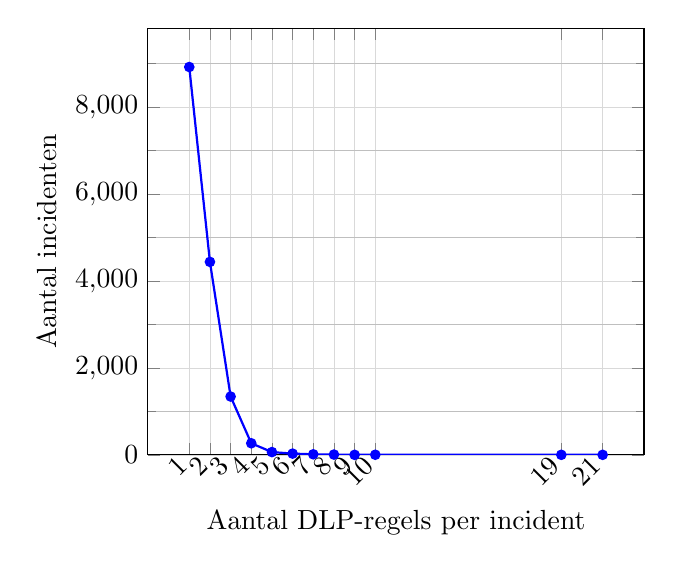
\begin{tikzpicture}
    \begin{axis}[
      xlabel={Aantal DLP-regels per incident},
      ylabel={Aantal incidenten},
      xtick={1,2,3,4,5,6,7,8,9,10,19,21},
      xticklabels={1,2,3,4,5,6,7,8,9,10,19,21},
      x tick label style={rotate=45,anchor=east},
      ymin=0,
      width=0.65\textwidth,     % maak de figuur smaller
      height=7cm,             % minder hoog
      mark size=1.5pt,          % kleinere puntjes
      grid=both,
      major grid style={line width=.2pt,draw=gray!30},
      minor tick num=1
    ]
      \addplot[
        thick,
        color=blue,
        mark=*,
      ]
      coordinates {
        (1,8921) (2,4439) (3,1342) (4,267)
        (5,64) (6,29) (7,13) (8,7)
        (9,1) (10,3) (19,1) (21,1)
      };
    \end{axis}
  \end{tikzpicture}
  \caption{Verdeling van aantal DLP-regels per incident}
  \label{fig:dlp-incidents-per-rule}
\end{figure}

\begin{figure}[H]
  \centering
  \scriptsize
  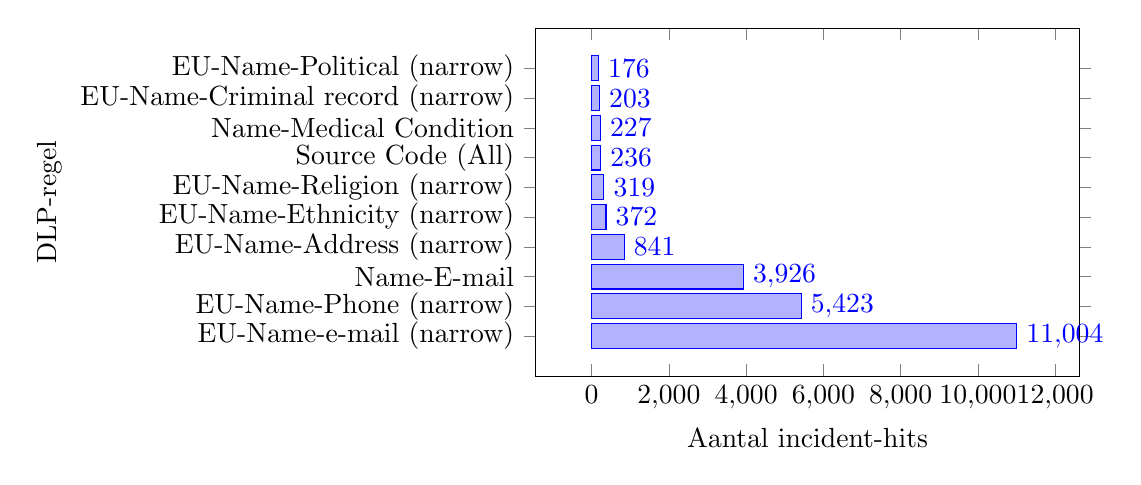
\begin{tikzpicture}
    \begin{axis}[
      xbar,
      bar width=9pt,
      enlargelimits=0.15,
      xlabel={Aantal incident-hits},
      ylabel={DLP-regel},
      ytick=data,
      yticklabels={
        EU-Name-e-mail (narrow),
        EU-Name-Phone (narrow),
        Name-E-mail,
        EU-Name-Address (narrow),
        EU-Name-Ethnicity (narrow),
        EU-Name-Religion (narrow),
        Source Code (All),
        Name-Medical Condition,
        EU-Name-Criminal record (narrow),
        EU-Name-Political (narrow)
      },
      nodes near coords,
      nodes near coords align={horizontal},
      scaled x ticks=false,
      xticklabel style={/pgf/number format/fixed},
      width=0.7\textwidth,
      height=6cm,
    ]
      \addplot coordinates {
        (11004,0) (5423,1) (3926,2) (841,3) (372,4)
        (319,5) (236,6) (227,7) (203,8) (176,9)
      };
    \end{axis}
  \end{tikzpicture}
  \caption{Top 10 DLP-regels met meeste incidenten}
  \label{fig:top10-dlprules}
\end{figure}


% \begin{figure}[H]
%   \centering
%   \scriptsize
%   \begin{tikzpicture}
%     \begin{axis}[
%       xbar,
%       bar width=10pt,
%       enlargelimits=0.15,
%       xlabel={Aantal incident-hits},
%       ylabel={DLP-regel},
%       ytick=data,
%       yticklabels={
%         EU-Name-e-mail (narrow),
%         EU-Name-Phone (narrow),
%         Name-E-mail,
%         EU-Name-Address (narrow),
%         EU-Name-Ethnicity (narrow),
%         EU-Name-Religion (narrow),
%         Source Code (All),
%         Name-Medical Condition,
%         EU-Name-Criminal record (narrow),
%         EU-Name-Political (narrow)
%       },
%       nodes near coords,
%       nodes near coords align={horizontal},
%       scaled x ticks=false,
%       xticklabel style={/pgf/number format/fixed},
%       width=0.8\textwidth,
%       height=8cm,
%     ]
%       \addplot coordinates {
%         (11004,0) (5423,1) (3926,2) (841,3) (372,4)
%         (319,5) (236,6) (227,7) (203,8) (176,9)
%       };
%     \end{axis}
%   \end{tikzpicture}
%   \caption{Top 10 DLP-regels met meeste incidenten}
%   \label{fig:top10-dlprules}
% \end{figure}



\begin{table}[H]
    \centering
    \small
    \scriptsize
    \begin{tabular}{ll}
        \toprule
        \textbf{Categorie} & \textbf{Waarde / Beschrijving} \\
        \midrule
        \multicolumn{2}{l}{\textbf{Overzicht incidenten}} \\
        Totaal aantal incidenten & 15.088 \\
        Totaal aantal gelogde berichten & 63.523 \\
        Gemiddeld aantal incidenten per bericht & $\approx$ 0,24 \\[4pt]

        \multicolumn{2}{l}{\textbf{Aantal DLP-regels per incident}} \\
        1 regel & 8.921 incidenten \\
        2 regels & 4.439 incidenten \\
        3 regels & 1.342 incidenten \\
        4 regels & 267 incidenten \\
        5 regels & 64 incidenten \\
        6 regels & 29 incidenten \\
        7 regels & 13 incidenten \\
        8 regels & 7 incidenten \\
        9 regels & 1 incident \\
        10 regels & 3 incidenten \\
        19 regels & 1 incident \\
        21 regels & 1 incident \\[4pt]

        \multicolumn{2}{l}{\textbf{Meest getroffen DLP-regels (top 10)}} \\
        EU-Name-e-mail (narrow) & 11.004 keer \\
        EU-Name-Phone (narrow) & 5.423 keer \\
        Name-E-mail & 3.926 keer \\
        EU-Name-Address (narrow) & 841 keer \\
        EU-Name-Ethnicity (narrow) & 372 keer \\
        EU-Name-Religion (narrow) & 319 keer \\
        Source Code (All) & 236 keer \\
        Name-Medical Condition & 227 keer \\
        EU-Name-Criminal record (narrow) & 203 keer \\
        EU-Name-Political (narrow) & 176 keer \\
        \bottomrule
    \end{tabular}
    \caption{Overzicht van Netskope DLP-incidenten en DLP-regels}
    \label{tab:netskope_dlp_resultaten}
\end{table}

Aangezien de e-mail dataset van \textit{Enron} afkomstig is van een \textbf{Amerikaanse} organisatie, 
zullen eigen gedefinieerde DLP-regels zoals \texttt{BE-National-ID (RRN)}~\ref{tab:custom-dlp-profielen} niet voorkomen in de incidenten.
Deze regels zijn specifiek gericht op Belgische identificatiegegevens.



\subsection{\IfLanguageName{dutch}{Overtredingen per incident}{Violations per DLP rule}}
\label{subsec:dlp-violations-per-rule}


Van de \textbf{15.088} incidenten zijn \textbf{306.403} overtredingen geregistreerd.
Figuur~\ref{fig:top-10-dlp-rules} en tabel~\ref{tab:dlp-severity-breakdown} tonen de tien DLP-regels met het hoogste aantal geregistreerde overtredingen door Netskope. 
Van de \textbf{306.403} overtredingen zijn \textbf{253.507} overtredingen afkomstig van de \texttt{EU-Name-e-mail (narrow)} en \texttt{Name-E-mail} regels.
Dit komt doordat sommige e-mails naar meerdere klanten en medewerkers worden verstuurd, waardoor elk e-mailadres in de e-mail wordt gezien als een aparte overtreding.
Bij de overige e-mails die niet gedetecteerd zijn, had Netskope niet genoeg reden om dit incident te registreren, 
waarschijnlijk doordat de gebruikersvertrouwensindex (\gls{uci}) nog hoog genoeg stond, zoals te zien in figuur~\ref{fig:netskope_user_info}.


\begin{figure}[H]
  \centering
  \scriptsize
  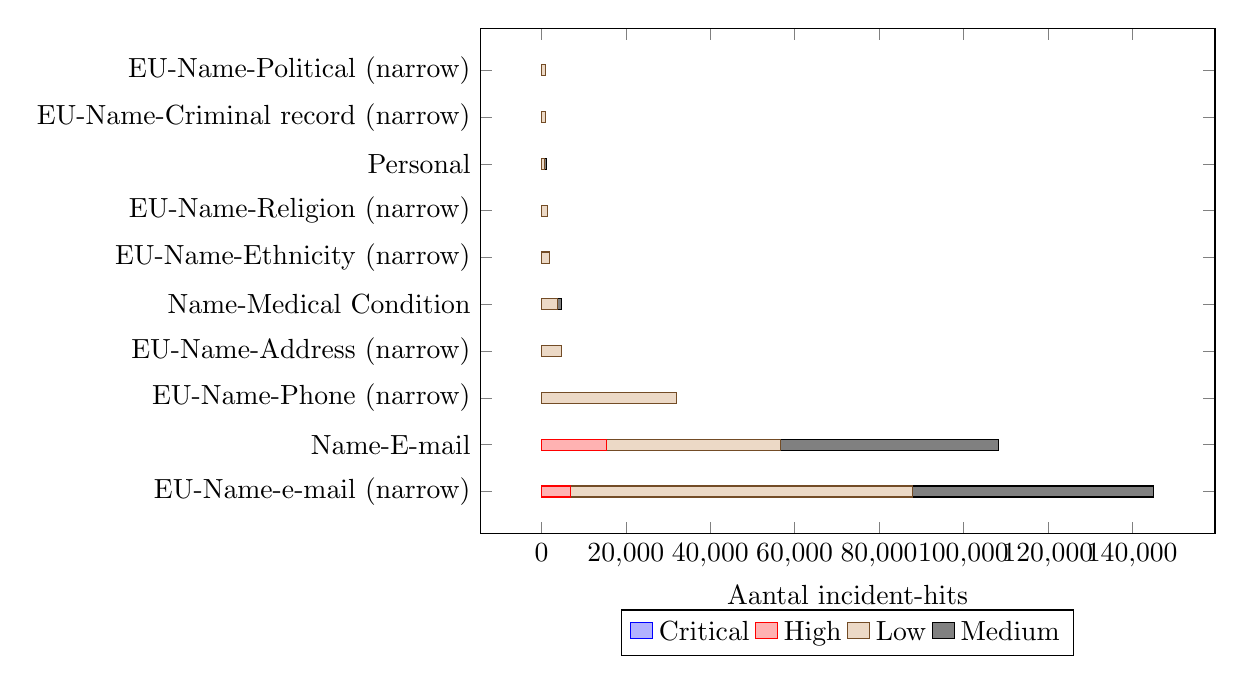
\begin{tikzpicture}
    \begin{axis}[
      xbar stacked,
      bar width=4pt,
      xlabel={Aantal incident-hits},
      ytick=data,
      yticklabels={
        EU-Name-e-mail (narrow),
        Name-E-mail,
        EU-Name-Phone (narrow),
        EU-Name-Address (narrow),
        Name-Medical Condition,
        EU-Name-Ethnicity (narrow),
        EU-Name-Religion (narrow),
        Personal,
        EU-Name-Criminal record (narrow),
        EU-Name-Political (narrow)
      },
      xticklabel style={/pgf/number format/fixed},
      scaled x ticks=false,
      legend style={at={(0.5,-0.15)}, anchor=north, legend columns=4},
      width=0.9\textwidth,
      height=8cm,
    ]
      % Critical
      \addplot+[xbar] coordinates {
        (0,0) (0,1) (0,2) (0,3) (0,4)
        (0,5) (0,6) (0,7) (0,8) (0,9)
      };
      % High
      \addplot+[xbar] coordinates {
        (6872,0) (15434,1) (0,2) (0,3) (0,4)
        (0,5) (0,6) (0,7) (0,8) (0,9)
      };
      % Low
      \addplot+[xbar] coordinates {
        (81040,0) (41178,1) (31988,2) (4772,3) (3888,4)
        (1930,5) (1488,6) (682,7) (954,8) (900,9)
      };
      % Medium
      \addplot+[xbar] coordinates {
        (57190,0) (51793,1) (0,2) (0,3) (853,4)
        (0,5) (0,6) (419,7) (0,8) (0,9)
      };
      \legend{Critical, High, Low, Medium}
    \end{axis}
  \end{tikzpicture}
  \caption{Top 10 DLP-regels met meeste overtredingen}
  \label{fig:top-10-dlp-rules}
\end{figure}

\begin{table}[H]
  \centering
  \scriptsize
  \begin{tabular}{lrrrrr}
    \toprule
    \textbf{DLP-Regel} & \textbf{Critical} & \textbf{High} & \textbf{Low} & \textbf{Medium} & \textbf{Totaal} \\
    \midrule
    EU-Name-e-mail (narrow)     & 0 & 6872  & 81040 & 57190 & 145102 \\
    Name-E-mail                 & 0 & 15434 & 41178 & 51793 & 108405 \\
    EU-Name-Phone (narrow)     & 0 & 0     & 31988 & 0     & 31988 \\
    EU-Name-Address (narrow)   & 0 & 0     & 4772  & 0     & 4772 \\
    Name-Medical Condition     & 0 & 0     & 3888  & 853   & 4741 \\
    EU-Name-Ethnicity (narrow) & 0 & 0     & 1930  & 0     & 1930 \\
    EU-Name-Religion (narrow)  & 0 & 0     & 1488  & 0     & 1488 \\
    Personal                   & 0 & 0     & 682   & 419   & 1101 \\
    EU-Name-Criminal record (narrow) & 0 & 0 & 954  & 0     & 954 \\
    EU-Name-Political (narrow) & 0 & 0     & 900   & 0     & 900 \\
    \bottomrule
  \end{tabular}
  \caption{Top 10 regels op basis van incident-hits}
  \label{tab:dlp-severity-breakdown}
\end{table}


\section{\IfLanguageName{dutch}{DLP-regels}{Predefined DLP rules vs Custom DLP rules}}
\label{sec:res-vooraf-gedefinieerde-dlp-regels}
% Vooraf gedefinieerde DLP-regels vs Eigen gedefinieerde DLP-regels

Zoals te zien in figuur~\ref{fig:netskope_rules} zijn 7 \textit{Real-Time Protection} DLP-beleiden aangemaakt in Netskope. 
Deze regels worden tijdens Netskope's evaluatie van boven naar beneden bekeken.
Eens een regel een match heeft gevonden, worden de onderstaande regels niet meer bekeken.
Aangezien het \textbf{\texttt{DLP-Predefined}}-beleid bovenaan staat en alle door Netskope gedefinieerde DLP-regels bevat, kwam het aantal incidenten altijd hierbij terecht.
\texttt{DLP-Predefined} en \texttt{DLP-GDPR} bevatten bijvoorbeeld beiden dezelfde \texttt{EU-Name-e-mail (narrow)} regel, maar doordat \texttt{DLP-Predefined} bovenaan staat, zal deze regel altijd enkel matchen op de \texttt{DLP-Predefined} regel,
ook al is de threshold van \texttt{DLP-GDPR} lager.
De \texttt{Alerts} kolom geeft het aantal gegenereerde incidenten weer over de laatste 30 dagen, dit geldt per bericht.
\textbf{74.286} incidenten vonden plaats tijdens de evaluatieperiode. Dit is hoger dan de \textbf{15.088} incidenten die Netskope heeft geregistreerd, doordat een bericht \textbf{meerdere regels} kan matchen.
Verder kan een bericht ook meerdere keren dezelfde regel matchen.
% Al deze overtredingen komen op een totaal van \textbf{306.403} overtredingen uit.
Alle overtredingen samen, vormen een totaal van \textbf{306.403} overtredingen.
Alle testen gebeurden op de \textit{Ngrok}-website, hierdoor wordt in de \textit{Source} kolom steeds \texttt{Sites for DLP test} weergegeven.


\begin{figure}[H]
    \centering
    \scriptsize
    \includegraphics[width=0.99\textwidth]{img/netskope_rules.png}
    \caption{Overzicht van aangemaakte \textit{Real-Time Protection} DLP-beleiden in Netskope}
    \label{fig:netskope_rules}
\end{figure}





% \section{\IfLanguageName{dutch}{Functionaliteit}{Functionality}}
% \label{sec:functionaliteit-resultaten}



\section{\IfLanguageName{dutch}{Correctheid}{Correctness}}
\label{sec:correctheid-resultaten}

Aansluitend aan sectie~\ref{sec:correctheid} zal de correctheid van de DLP-regels worden geëvalueerd aan de hand van een confusion matrix~\ref{tab:confusion_matrix}. 
Tabel~\ref{tab:confusion_matrix-resultaten} toont de confusion matrix voor de vooraf gedefinieerde DLP-regels. 
De evaluatieperiode omvatte 22 april 2025 tot en met 25 mei 2025. 
Gedurende de feedback periode met de werknemers van Evolane kwamen \textbf{231} verschillende incidenten binnen, verspreid over \textbf{3} weken. 
Deze kwamen van \textbf{4} verschillende medewerkers, \textbf{3} hiervan waren van het \textit{Sales} team en \textbf{1} van het \textit{Security} team.
\textit{Sales} medewerkers werken voornamelijk met vertrouwelijke klantendocumenten, hierdoor zal deze data niet geanalyseerd opgevraagd worden.
De regels die werden gedetecteerd, lijken overeen te komen met wat in een klantendossier zou staan, zoals bijvoorbeeld een \texttt{EU-Name-e-mail} of \texttt{EU-Name-phone}.

De evaluatie van \textbf{\textit{Enron}}-data werd uitgevoerd van \textbf{18} tot en met \textbf{25} mei 2025.
Hiervan werden \textbf{100} e-mails steekproefsgewijs geanalyseerd, 
met de selectie van \textbf{50} e-mails met confidentiële data en \textbf{50} e-mails zonder confidentiële data.
% waarbij rekening werd gehouden om \textbf{50} e-mails te selecteren die volgens Netskope confidentiële data bevatten en \textbf{50} e-mails zonder confidentiële data.
Verder werd bij de confidentiële incidenten gekeken naar verschillende geregistreerde DLP-regels die Netskope heeft aangemaakt.
Dit komt doordat de regel \texttt{EU-Name-e-mail}, zoals verwacht, frequent voor zou komen in een dataset van e-mails.
Dit staat in tabel~\ref{tab:confusion_matrix-resultaten} weergegeven.


\begin{table}[h]
    \centering
    \small
    \scriptsize
    \begin{tabular}{|c|c|c|c|}
        \hline
        \textbf{} & \textbf{Werkelijke Gevoelige Data} & \textbf{Geen Gevoelige Data} & \textbf{Totaal} \\ \hline
        \textbf{Gedetecteerd als gevoelig} & \textbf{39} (TP) & \textbf{11} (FP) & 50 \\ \hline
        \textbf{Niet gedetecteerd als gevoelig} & \textbf{0} (FN) & \textbf{50} (TN) & 50 \\ \hline
    \end{tabular}
    \caption{Confusion Matrix met 10\% gevoelige data en 11 false positives}
    \label{tab:confusion_matrix-resultaten}
\end{table}


Aangezien de identificatiegegevens van de DLP-regels niet publiek beschikbaar zijn bij vooraf gedefinieerde DLP-identificatiegegevens,
is het zoeken naar false positives giswerk. Hierdoor werd gezocht naar directe overeenkomsten die mogelijks met de regels overeenkomen.
Voor volgende \textbf{11} is dit niet gelukt en kwamen ze daarbij in de \textit{False Positive} categorie terecht:

\begin{table}[H]
  \centering
  \begin{tabular}{lr}
    \toprule
    \textbf{Detectietype} & \textbf{Aantal false positives} \\
    \midrule
    \texttt{Source code}                & 2 \\
    \texttt{EU-Name-e-mail}             & 2 \\
    \texttt{EU-Name-Religion (narrow)} & 2 \\
    \texttt{Blasphemous}               & 1 \\
    \texttt{AU-PAN-Exp-Name}           & 1 \\
    \texttt{COL-Name-Birth}            & 1 \\
    \texttt{EU-Identity-Ethnicity}     & 1 \\
    \texttt{EU-Name-Gender (narrow)}   & 1 \\
    \bottomrule
  \end{tabular}
  \caption{Overzicht van false positives per detectietype}
  \label{tab:false-positives}
\end{table}


\textit{False Negatives} zijn niet ontdekt, alle bekeken e-mails zonder confidentiële data hadden dit niet.

\textcite{Quaeyhaegens2025}, \textit{Partner Solution Architect} bij \textbf{Netskope}, verklaarde tijdens \textit{Cybersec Europe}:
% ``Netskope DLP-incidenten kunnen false positives bevatten, maar genereren nooit false negatives''. 

\begin{quote}
\textit{``Netskope DLP-incidenten kunnen false positives bevatten, maar genereren nooit false negatives''}
\end{quote}

Deze uitspraak is een persoonlijke notitie. 
DLP-systemen detecteren uitsluitend gegevens die voldoen aan gedefinieerde regels, waardoor relevante matches altijd in beeld komen zolang de configuratie correct blijft.
Dit onderbouwt de resultaten van de tabel~\ref{tab:confusion_matrix-resultaten}, waar geen false negatives zijn gevonden.


% \begin{table}[H]
%     \centering
%     \small
%     \scriptsize
%     \begin{tabular}{|c|c|c|}
%         \hline
%         \textbf{} & \textbf{Werkelijke Gevoelige Data} & \textbf{Geen Gevoelige Data} \\ \hline
%         \textbf{Gedetecteerd als gevoelig} & \textbf{} (TP) & \textbf{} (FP) \\ \hline
%         \textbf{Niet gedetecteerd als gevoelig} & \textbf{} (FN) & \textbf{} (TN) \\ \hline
%     \end{tabular}
%     \caption{Confusion Matrix voor regex-detectie}
%     \label{tab:confusion_matrix}
% \end{table}


% \subsection{\IfLanguageName{dutch}{Correctheid}{Correctness}}
% \label{sec:correctheid-resultaten-eigen}

% \textcite{Quaeyhaegens2025}, \textit{Partner Solution Architect} bij \textbf{Netskope}, verklaarde tijdens \textit{Cybersec Europe}:
% ``Netskope DLP-incidenten kunnen false positives bevatten, maar genereren nooit false negatives''. 

% \begin{quote}
% \textit{``Netskope DLP-incidenten kunnen false positives bevatten, maar genereren nooit false negatives''}
% \end{quote}

% Deze uitspraak is een persoonlijke notitie. 
% DLP-systemen detecteren uitsluitend gegevens die voldoen aan gedefinieerde regels, waardoor relevante matches altijd in beeld komen zolang de configuratie correct blijft.

% % Quaeyhaegens2025


% \begin{table}[h]
%     \centering
%     \small
%     \scriptsize
%     \begin{tabular}{|c|c|c|}
%         \hline
%         \textbf{} & \textbf{Werkelijke Gevoelige Data} & \textbf{Geen Gevoelige Data} \\ \hline
%         \textbf{Gedetecteerd als gevoelig} & TP & FP \\ \hline
%         \textbf{Niet gedetecteerd als gevoelig} & FN & TN \\ \hline
%     \end{tabular}
%     \caption{Confusion Matrix voor regex-detectie}
%     \label{tab:confusion_matrix-eigen}
% \end{table}

\section{\IfLanguageName{dutch}{Performantie}{Performance}}
\label{sec:performantie-resultaten}
% {sec:eva-performantie}

Om de impact van de Netskope agent op de netwerkperformantie te evalueren, werd gebruik gemaakt van de tool \textbf{iPerf3}.
De tests werden uitgevoerd op een \textit{macOS}-systeem, met telkens een client-verbinding naar een publieke \textit{iperf3}-server.
Netskope \textbf{\textit{blokkeerde de verbinding}} naar de publieke \textit{iperf3}-server, waardoor de tests niet konden doorgaan.
Dit komt doordat Netskope al eerder was geconfigureerd. Tijdens de tests was geen mogelijkheid tot het specifiek toestaan van \textit{iperf3}-verkeer.
%om specifiek het \textit{iperf3}-verkeer toe te staan.

Perfomantietests werden dus enkel uitgevoerd met \textit{macOS} \texttt{Activity Monitor}.
Hierbij bleek echter dat de Netskope agent geen merkbare impact had op de netwerkperformantie, zoals eerder vermeld in sectie~\ref{sec:eva-performantie}~\autocite{Netskope2025Utilization}.

% Om de impact van de Netskope-agent op de netwerkperformantie te evalueren, werd gebruik gemaakt van de tool \texttt{iPerf3}. 
% De tests werden uitgevoerd op een macOS-systeem, met telkens een client-verbinding naar een publieke \texttt{iperf3}-server. 

% Elke test liep gedurende 60 seconden met een logging-interval van 5 seconden. Onderstaande tabel toont de gemiddelde throughput en eventuele merkbare vertraging.
% De testscenario's~\ref{tab:test-scenarios-performance} gaven volgende resultaten:

% % % % % % % Tijdens de test met actieve agent werd ook het netwerkverkeer geanalyseerd via \texttt{Wireshark}. 
% % % % % % % Hieruit blijkt dat de agent actief verbindingen intercept via een lokale proxy (TCP verbinding naar \texttt{127.0.0.1:port}) alvorens verkeer door te sturen. 
% % % % % % % Deze interceptie introduceert merkbare vertraging bij uploads van gevoelige bestanden, wat zichtbaar is in de lagere throughput en hogere latency. 
% % % % % % % % \item Wireshark bevestigde TLS-interceptie bij upload van een testbestand met dummy persoonsgegevens.

%  .\iperf3.exe -s
% ngrok tcp 5201 


% \begin{table}[h]
%     \centering
%     \begin{tabular}{lcc}
%         \toprule
%         \textbf{Testscenario} & \textbf{Gemiddelde download (Mbps)} & \textbf{Retransmissies} \\
%         \midrule
%         Zonder Netskope             & 94.5 & 0 \\
%         Met Netskope (passief)      & 89.2 & 1 \\
%         Met Netskope (DLP actief)   & 74.8 & 3 \\
%         Met Netskope (Tijdens upload) & 65.3 & 5 \\
%         \bottomrule
%     \end{tabular}
%     \caption{Netwerkperformance met en zonder Netskope (gemeten via \texttt{iPerf3})}
%     \label{tab:iperf3-results}
% \end{table}

\subsection{\IfLanguageName{dutch}{Gebruiksvriendelijkheid}{User-friendliness}}
\label{sec:gebruiksvriendelijkheid-resultaten}

\subsubsection{\iflanguage{dutch}{Hoe eenvoudig is het om de DLP-regels te configureren?}{false}}

Tijdens de PoC was het eenvoudig om eigen gedefinieerde DLP-regels aan te maken.
Aangezien echter de vooraf gedefinieerde DLP-regels niet aanpasbaar zijn, is het moeilijk om deze regels te configureren.
% maar aangezien Netskope vooraf gedefinieerde DLP-regels die niet aanpasbaar zijn, is het moeilijk om deze regels te configureren.
De thresholds~\ref{tab:risico_thresholds_predefined} van deze regels staan vast, waardoor tijdens de PoC veel tijd is besteed aan het \textit{clonen} van de regels, zodat de thresholds wel konden worden aangepast.
De entiteiten van identificatiegegevens zijn niet publiek, waardoor het moeilijk is om te evalueren welke regels precies zijn en welke entiteiten Netskope gebruikt.
% Dit onderzoek probeerde 

% Aangezien deze regels vooraf zijn gedefinieerd, kan je dit direct toepassen op de organisatie. 
% is bijvoorbeeld geen mogelijkheid om de thresholds te veranderen. 
% Wat lastig kan zijn als je DLP regels wilt toepassen 

% 1. Niet aanpasbare profielen/regels (Geen mogelijkheid om thresholds te veranderen)
% 2. Entiteiten zijn niet publiek (moeilijk evalueren als je niet weet wat  mist)

\subsubsection{\iflanguage{dutch}{Is voldoende documentatie beschikbaar voor de DLP-regels?}{testttt}}

Ja, tijdens dit onderzoek is voldoende documentatie geraadpleegd op \textbf{Knowledge Base van \textcite{Netskope2025Docs}}
Deze documentatie bevat veel informatie over alle mogelijke features van Netskope, waaronder Data Loss Prevention.

\subsubsection{\iflanguage{dutch}{Hoe eenvoudig is het om de DLP-regels te gebruiken?}{false}}

De DLP-regels zijn eenvoudig te gebruiken, Netskope heeft een duidelijke interface waar je de regels kan beheren.
Eens een regel is aangemaakt en geactiveerd, zal Netskope deze onmiddellijk toepassen op al het ingestelde verkeer.

\subsubsection{\iflanguage{dutch}{Is voldoende ondersteuning beschikbaar voor de DLP-regels?}{false}}

% Ja, gemakkelijk te clonen om zelf regels aan te maken en aan te passen. 
Ja, het is eenvoudig om de DLP-regels te clonen en aan te passen.
Verder zijn de DLP-regels makkelijk aanpasbaar en worden deze direct toegepast op het verkeer.
Dit is ook een van de redenen waarom, zoals vermeld in sectie~\ref{sec:netskope-literatuurstudie}, Netskope zo hoog staat in de Magic Quadrant van \textcite{Gartner2024}.

% Top Alternatieven voor Netskope DLP
% https://www.nightfall.ai/blog/netskope-dlp-comprehensive-analysis-and-top-alternatives

% The Netskope client uses the same method to inspect and filter traffic that the GlobalProtect App uses to implement domain and application-based split tunneling. The Netskope client can prevent traffic from being sent out the correct interface (VPN virtual interface or physical interface).
% https://knowledgebase.paloaltonetworks.com/KCSArticleDetail?id=kA14u0000001VGGCA2&lang=en_US%E2%80%A9#:~:text=The%20Netskope%20client%20uses%20the,virtual%20interface%20or%20physical%20interface


% test2
% \begin{figure}[ht]
%   \centering
%   \tiny
%   \scriptsize            % Nog een stapje kleiner dan \scriptsize kun je \tiny proberen
%   \begin{tikzpicture}
%     \begin{axis}[
%       xbar,
%       bar width=8pt,      % smallere balken
%       enlarge y limits=0.3,
%       xlabel={Aantal incidenten},
%       ylabel={Combinatie van DLP-regels},
%       symbolic y coords={
%         {EU-Name-e-mail (narrow)},
%         {EU-Name-Phone (narrow)},
%         {EU-Name-e-mail (narrow),\,Name-E-mail},
%         {EU-Name-Phone (narrow),\,EU-Name-e-mail (narrow)},
%         {EU-Name-Phone (narrow),\,EU-Name-e-mail (narrow),\,Name-E-mail}
%       },
%       ytick=data,
%       yticklabel style={
%         align=left,
%         font=\scriptsize % labels in kleinere font
%       },
%       nodes near coords,
%       nodes near coords align={horizontal},
%       width=0.75\textwidth,  % minder breed
%       height=5cm,            % minder hoog
%       tick label style={font=\scriptsize},
%     ]
%       \addplot coordinates {
%         (5414,{EU-Name-e-mail (narrow)})
%         (2110,{EU-Name-Phone (narrow)})
%         (1905,{EU-Name-e-mail (narrow),\,Name-E-mail})
%         (1659,{EU-Name-Phone (narrow),\,EU-Name-e-mail (narrow)})
%         (721,{EU-Name-Phone (narrow),\,EU-Name-e-mail (narrow),\,Name-E-mail})
%       };
%     \end{axis}
%   \end{tikzpicture}
%   \caption{Top 5 meest voorkomende combinaties van DLP-regels}
%   \label{fig:top5-dlpcombos}
% \end{figure}


% \begin{figure}[ht]
%   \centering
%   \small
%   \scriptsize
%   \begin{tikzpicture}
%     \pie[
%       sum=100,            % de waarden tellen zelf op naar 100
%       radius=4,           % kleine radius
%       text=inside,        % zet label + percentage ín de slice
%       after number=\,\%,  % voeg %-teken toe
%       explode=0.1         % ietsjes het eerste segment uit elkaar
%     ]{
%       3.8/Incidenten,
%       16.1/Berichten,
%       77.3/Schendingen,
%       0.01/Profielen,
%       0.02/Regels
%     }
%   \end{tikzpicture}
%   \caption{Samenvattende statistieken (in \%)}
%   \label{fig:summary-pie}
% \end{figure}

% \begin{figure}[ht]
%   \centering
%   \begin{tikzpicture}
%     \pie[
%       radius=3,
%       text=legend,
%       before number=,
%       after number=\%,
%       sum=auto,
%       color={Rood, HogentBlauw, HogentLichtOranje, Groen, Paars}
%     ]{
%       3.92/Incidents (3.92\%),
%       16.49/Messages (16.49\%),
%       79.56/Violations (79.56\%),
%       0.0083/Profiles (0.0083\%),
%       0.0187/Rules (0.0187\%)
%     }
%   \end{tikzpicture}
%   \caption{Distribution of DLP-related data based on absolute numbers}
%   \label{fig:pie-overview}
% \end{figure}


% \begin{figure}[ht]
%   \centering
%   \scriptsize
%   \begin{tikzpicture}
%     \begin{axis}[
%       xbar stacked,
%       bar width=4pt,
%       xlabel={Aantal incident-hits},
%       ytick=data,
%       yticklabels={
%         EU-Name-e-mail (narrow),
%         Name-E-mail,
%         EU-Name-Phone (narrow),
%         EU-Name-Address (narrow),
%         EU-Name-Ethnicity (narrow),
%         EU-Name-Religion (narrow),
%         EU-Name-Criminal record (narrow),
%         EU-Name-Political (narrow),
%         Name-Medical Condition,
%         Personal
%       },
%       legend style={at={(0.5,-0.15)}, anchor=north, legend columns=4},
%       nodes near coords,
%       nodes near coords align={horizontal},
%       width=0.9\textwidth,
%       height=8cm,
%     ]
%       % Data: critical, high, low, medium (stacked per regel)
%       \addplot+[xbar] coordinates {
%         (0,0) (0,1) (0,2) (0,3) (0,4)
%         (0,5) (0,6) (0,7) (0,8) (0,9)
%       }; % Critical
%       \addplot+[xbar] coordinates {
%         (6872,0) (15434,1) (0,2) (0,3) (0,4)
%         (0,5) (0,6) (0,7) (0,8) (0,9)
%       }; % High
%       \addplot+[xbar] coordinates {
%         (81040,0) (41178,1) (31988,2) (4772,3) (1930,4)
%         (1488,5) (954,6) (900,7) (3888,8) (682,9)
%       }; % Low
%       \addplot+[xbar] coordinates {
%         (57190,0) (51793,1) (0,2) (0,3) (0,4)
%         (0,5) (0,6) (0,7) (853,8) (419,9)
%       }; % Medium
%       \legend{Critical, High, Low, Medium}
%     \end{axis}
%   \end{tikzpicture}
%   \caption{Top 10 DLP-regels met stacked severity breakdown}
%   \label{fig:stacked-dlp-top10}
% \end{figure}




% \begin{figure}[ht]
%   \centering
%   \begin{tikzpicture}
%     \pie[
%       radius=3,
%       text=legend,
%       before number=,
%       after number=\%,
%       sum=auto,
%       color={Rood, HogentBlauw, HogentOranje, Groen, Paars, HogentLichtBlauw, Geel, Roos, Lime, Grijs}
%     ]{
%       54.14/{EU-Name-e-mail (narrow)},
%       21.10/{EU-Name-Phone (narrow)},
%       19.05/{{EU-Name-e-mail (narrow), Name-E-mail}},
%       16.59/{{EU-Name-Phone (narrow), EU-Name-e-mail (narrow)}},
%       7.21/{{EU-Name-Phone (narrow), EU-Name-e-mail (narrow), Name-E-mail}},
%       5.78/{Name-E-mail},
%       1.82/{EU-Name-Address (narrow)},
%       1.41/{Source Code (All)},
%       1.21/{{EU-Name-Address (narrow), EU-Name-Phone (narrow)}},
%       1.16/{{EU-Name-Address (narrow), EU-Name-Phone (narrow), EU-Name-e-mail (narrow)}}
%     }
%   \end{tikzpicture}
%   \caption{Top 10 most common DLP rule combinations}
%   \label{fig:pie-dlp-rule-combos}
% \end{figure}

